%%%%%%%%%%%%%%%%%%%%%%%%%%%%%%%%%%%%%%%%%
% University Assignment Title Page 
% LaTeX Template
% Version 1.0 (27/12/12)
%
% This template has been downloaded from:
% http://www.LaTeXTemplates.com
%
% Original author:
% WikiBooks (http://en.wikibooks.org/wiki/LaTeX/Title_Creation)
%
% License:
% CC BY-NC-SA 3.0 (http://creativecommons.org/licenses/by-nc-sa/3.0/)
% 
% Instructions for using this template:
% This title page is capable of being compiled as is. This is not useful for 
% including it in another document. To do this, you have two options: 
%
% 1) Copy/paste everything between \begin{document} and \end{document} 
% starting at \begin{titlepage} and paste this into another LaTeX file where you 
% want your title page.
% OR
% 2) Remove everything outside the \begin{titlepage} and \end{titlepage} and 
% move this file to the same directory as the LaTeX file you wish to add it to. 
% Then add \input{./title_page_1.tex} to your LaTeX file where you want your
% title page.
%
%%%%%%%%%%%%%%%%%%%%%%%%%%%%%%%%%%%%%%%%%
%\title{Title page with logo}
%----------------------------------------------------------------------------------------
%	PACKAGES AND OTHER DOCUMENT CONFIGURATIONS
%----------------------------------------------------------------------------------------

\documentclass[12pt]{article}
\usepackage[english]{babel}
\usepackage[utf8x]{inputenc}
\usepackage{amsmath}
\usepackage{graphicx}
\usepackage{float}
\usepackage{listings}
\usepackage[colorinlistoftodos]{todonotes}
\usepackage{textcomp}

\usepackage{geometry}
 \geometry{
 a4paper,
 total={170mm,257mm},
 left=20mm,
 top=20mm,
 }
 
 % Better inline directory listings
\usepackage{xcolor}
\definecolor{light-gray}{gray}{0.95}
\newcommand{\code}[1]{\colorbox{light-gray}{\texttt{#1}}}

% Paragraph formatting
\setlength{\parindent}{0em}
\setlength{\parskip}{1em}

% Subsubsubsection
% \usepackage{titlesec}
% \setcounter{secnumdepth}{4}
% \titleformat{\paragraph}
% {\normalfont\normalsize\bfseries}{\theparagraph}{1em}{}
% \titlespacing*{\paragraph}
% {0pt}{3.25ex plus 1ex minus .2ex}{1.5ex plus .2ex}

\usepackage{titlesec}
\usepackage{hyperref}

\titleclass{\subsubsubsection}{straight}[\subsection]

\newcounter{subsubsubsection}[subsubsection]
\renewcommand\thesubsubsubsection{\thesubsubsection.\arabic{subsubsubsection}}
\renewcommand\theparagraph{\thesubsubsubsection.\arabic{paragraph}} % optional; useful if paragraphs are to be numbered

\titleformat{\subsubsubsection}
  {\normalfont\normalsize\bfseries}{\thesubsubsubsection}{1em}{}
\titlespacing*{\subsubsubsection}
{0pt}{3.25ex plus 1ex minus .2ex}{1.5ex plus .2ex}

\makeatletter
\renewcommand\paragraph{\@startsection{paragraph}{5}{\z@}%
  {3.25ex \@plus1ex \@minus.2ex}%
  {-1em}%
  {\normalfont\normalsize\bfseries}}
\renewcommand\subparagraph{\@startsection{subparagraph}{6}{\parindent}%
  {3.25ex \@plus1ex \@minus .2ex}%
  {-1em}%
  {\normalfont\normalsize\bfseries}}
\def\toclevel@subsubsubsection{4}
\def\toclevel@paragraph{5}
\def\toclevel@paragraph{6}
\def\l@subsubsubsection{\@dottedtocline{4}{7em}{4em}}
\def\l@paragraph{\@dottedtocline{5}{10em}{5em}}
\def\l@subparagraph{\@dottedtocline{6}{14em}{6em}}

% Format of references to sections
\AtBeginDocument{%
  \@ifdefinable{\myorg@nameref}{%
    \LetLtxMacro\myorg@nameref\nameref
    \DeclareRobustCommand*{\nameref}[1]{%
      \emph{\myorg@nameref{#1}}%
    }%
  }%
}


\makeatother

\setcounter{secnumdepth}{4}
\setcounter{tocdepth}{4}

\begin{document}
\textwidth=15cm

\lstset{language=C++,
                basicstyle=\fontsize{10}{10}\ttfamily,
                keywordstyle=\color{blue}\ttfamily,
                stringstyle=\color{red}\ttfamily,
                commentstyle=\color{gray!80}\ttfamily,
                morecomment=[l][\color{magenta}]{\#}
}

\begin{titlepage}

\newcommand{\HRule}{\rule{\linewidth}{0.5mm}} % Defines a new command for the horizontal lines, change thickness here

\center % Center everything on the page
 
%----------------------------------------------------------------------------------------
%	HEADING SECTIONS
%----------------------------------------------------------------------------------------

\textsc{\LARGE Politenico di Milano}\\[1.5cm] % Name of your university/college
\textsc{\Large Dipartimento Elettronica, Informazione e Bioingegneria}\\[0.5cm] % Major heading such as course name
\textsc{\large HEAPLab Project Report}\\[0.5cm] % Minor heading such as course title

%----------------------------------------------------------------------------------------
%	TITLE SECTION
%----------------------------------------------------------------------------------------

\HRule \\[0.4cm]
{ \huge \bfseries Digital Audio Effects}\\[0.4cm] % Title of your document
\HRule \\[1.5cm]
 
%----------------------------------------------------------------------------------------
%	AUTHOR SECTION
%----------------------------------------------------------------------------------------

\begin{minipage}{0.4\textwidth}
\begin{flushleft} \large
\emph{Authors:}\\
Generoso \textsc{Imparato} \newline
Yazan \textsc{Matar}
\end{flushleft}
\end{minipage}
~
\begin{minipage}{0.4\textwidth}
\begin{flushright} \large
\emph{Supervisor:} \\
Federico \textsc{Terraneo} % Supervisor's Name
\end{flushright}
\end{minipage}\\[2cm]

% If you don't want a supervisor, uncomment the two lines below and remove the section above
%\Large \emph{Author:}\\
%John \textsc{Smith}\\[3cm] % Your name

%----------------------------------------------------------------------------------------
%	DATE SECTION
%----------------------------------------------------------------------------------------

{\large \today}\\[2cm] % Date, change the \today to a set date if you want to be precise

%----------------------------------------------------------------------------------------
%	LOGO SECTION
%----------------------------------------------------------------------------------------


\includegraphics[width=100pt]{img/heaplogo.pdf}\\[1cm] % Include a department/university logo - this will require the graphicx package

\emph{Github repo:}\\
\href{https://github.com/GenniImparato/Digital\_Audio\_Effect}{https://github.com/GenniImparato/Digital\_Audio\_Effect}\par
 
%----------------------------------------------------------------------------------------

\vfill % Fill the rest of the page with whitespace

\end{titlepage}

\tableofcontents
\newpage


\section{Introduction}
\label{sec:Intro}

The aim of this project is to create a platform to experiment with real-time DSP effects on audio, with an STM32 microprocessor, using a multi-threaded, real-time environment. \\
We designed an audio chain system with the following specifications:

\begin{itemize}
    \item Input audio can be selected from two sources:
        \begin{itemize}
          \item Audio sampled from an analog audio signal coming from a jack connector
          \item Audio generated by a software audio synthesizer
        \end{itemize}
    \item Audio stream coming from the selected source can be sent through different selectable DSP effects 
    \item Output audio can be heard in real-time with a speaker, as well as earphones through the jack connector
    \item Synthesizer, as well as the effects, has parameters that can be changed in real-time.
\end{itemize}

To realize such functionalities, and to better visualize, hear, and control the system, we designed an auxiliary PCB with extra hardware which will be described in detail in the relative section.

\newpage

\section{Design and Implementation}
\label{sec:Design}
In this section we describe the hardware components and functionalities as well as the software implementation and how those components interact with one another.

\subsection{Hardware}
\label{sec:HW}
In the following sections we analyze in detail the hardware components used for this project, which are the \textbf{STM32F407 Discovery Board} and the \textbf{custom PCB} designed to improve the user experience.

\subsubsection{STM32F407 Discovery Board}
The microcontroller used for the project is the
STM32F407 Discovery Board, which offers (mainly for this project) the following features:

\begin{itemize}
    \item STM32F407VGT6 microcontroller featuring 32-bit Arm\textsuperscript{\textregistered} Cortex\textsuperscript{\textregistered}-M4 with FPU core
    \item 1-Mbyte Flash memory and 192-Kbyte RAM
    \item Audio DAC with integrated class D speaker driver
    \item User and reset push-buttons
    \item Stereo headphone output jack
    \item External application power supply: 3V and 5V
\end{itemize}
For more specifications about the board, read the datasheet and the user manual or go to the manufacturer website.

\subsubsection{Custom PCB}
\label{sec:PCB}
We designed a PCB in Eagle with connectors to insert the STM32F407 discovery board.
The PCB contains extra hardware useful for the project, such as:
\begin{itemize}
    \item Speaker with an amplifier circuit
    \item Audio buffer for ADC sampling
    \item Led matrix [10x15]
    \item Linear potentiometers (for effect controls)
    \item Logarithmic potentiometer (for amplifier volume)
    \item External power supply
\end{itemize}

Details on the PCB are shown in the next sections.

\subsubsubsection{Circuits}
\label{sec:Circuit}

    \begin{figure}[H]
      \centering
        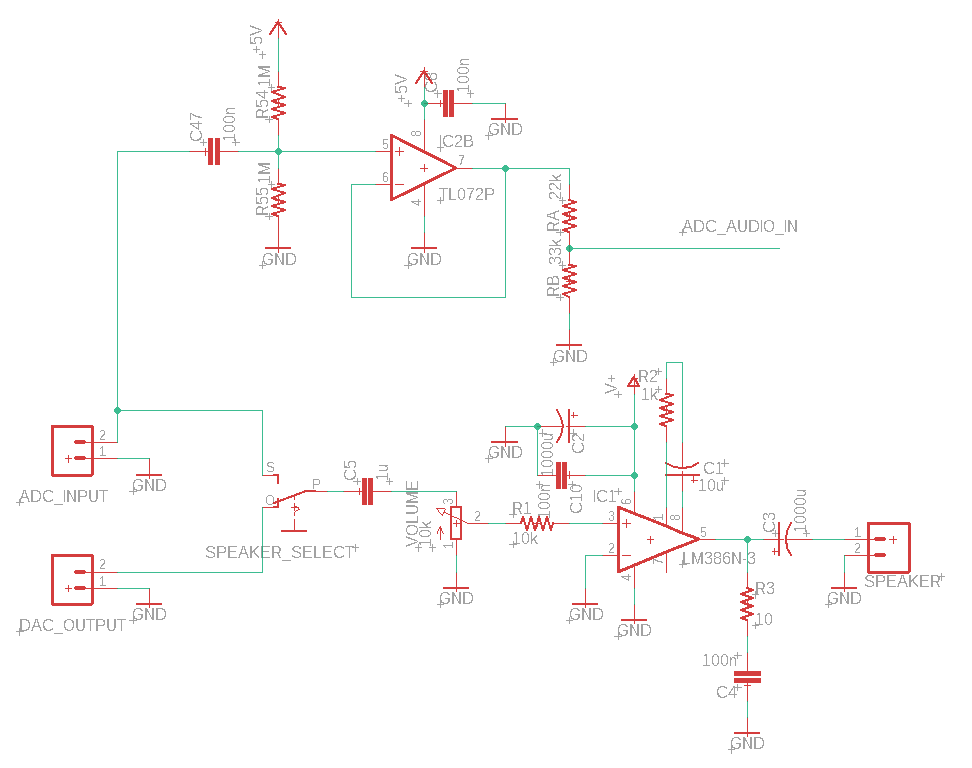
\includegraphics[width=\textwidth]{img/audio.png}
        \caption{Audio circuit}
    \end{figure}
    
    This circuit contains a buffer between the input analog audio signal and the STM32 internal ADC input.\\
    The signal is shifted in range from 0 to 3.3V and centered around 1.65 V to be sampled by the ADC.\\
    It also contains the amplifier circuit that drives the 8 ohm speaker on the board, including a volume potentiometer. \\
    The input of the speaker amplifier can be selected with a switch between the raw input audio and the DAC output of the discovery board.
    
    \begin{figure}[H]
      \centering
        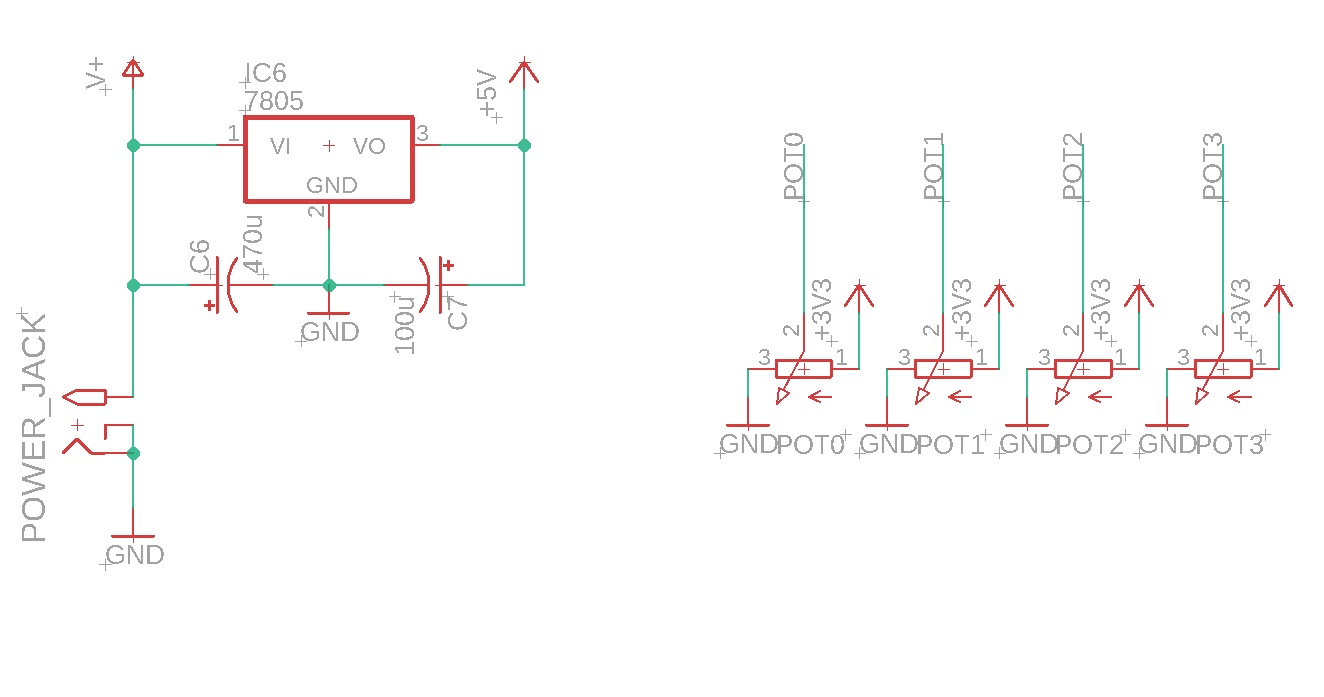
\includegraphics[width=\textwidth]{img/power.png}
        \caption{Power and potentiometers circuit}
    \end{figure}
    
    The input voltage from the power is applied directly to the speaker amplifier power supply, while the voltage for the discovery board is obtained by a 5V voltage regulator.
    
    \begin{figure}[H]
      \centering
        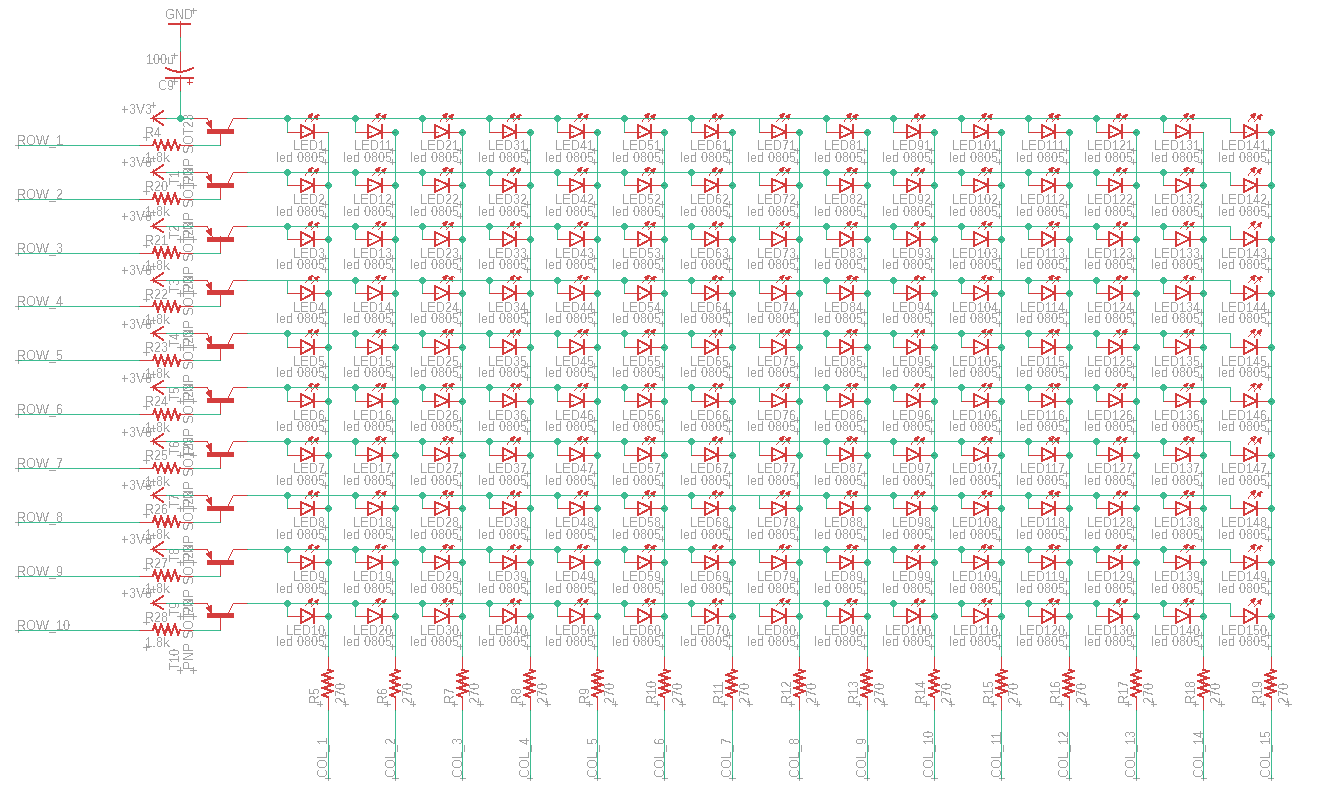
\includegraphics[width=\textwidth]{img/ledmatrix.png}
        \caption{Led matrix circuit}
    \end{figure}
    
    The led matrix is made with 150 SMD leds, divided in 10 rows and 15 columns.\\
    Each row is controlled by a PNP transistor with the base connected to a GPIO pin of the discovery board. Columns are connected directly to GPIO pins.
    
    \begin{figure}[H]
      \centering
        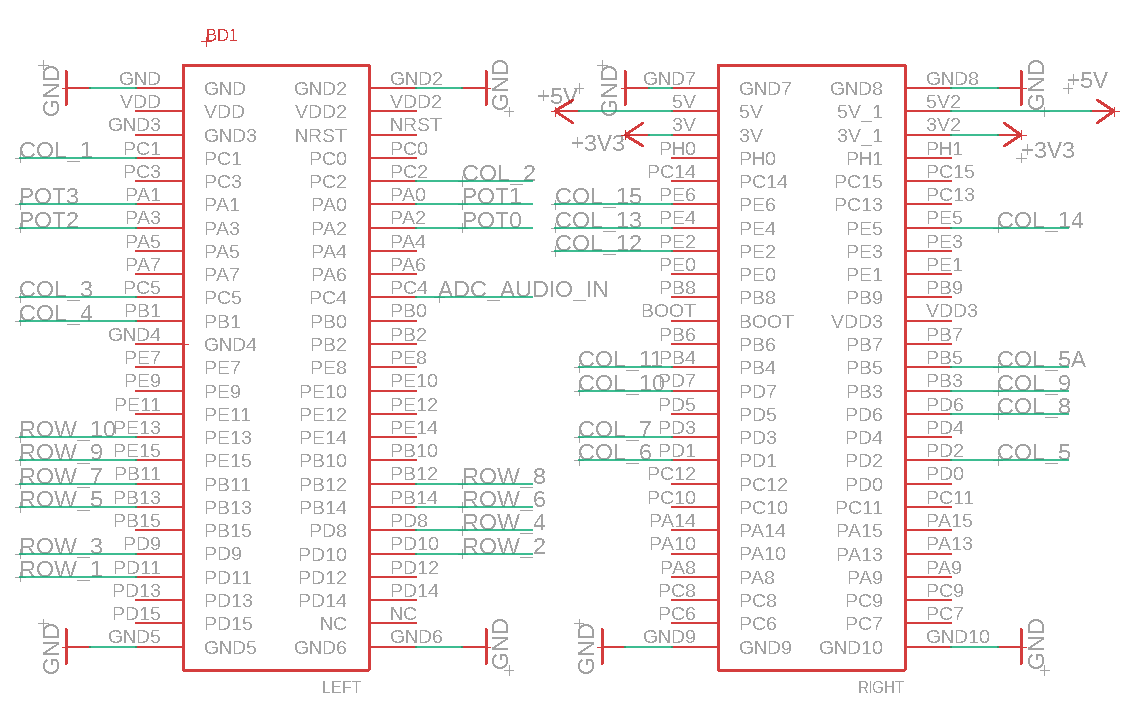
\includegraphics[width=\textwidth]{img/stm32.png}
        \caption{STM32F407 Discovery Board connectors}
    \end{figure}
    
    This connectors allow to easily insert and remove the STM32F407 Discovery Board from the PCB.

\newpage
\subsubsubsection{Layout}
\label{sec:Layout}
    
    \begin{figure}[H]
      \centering
        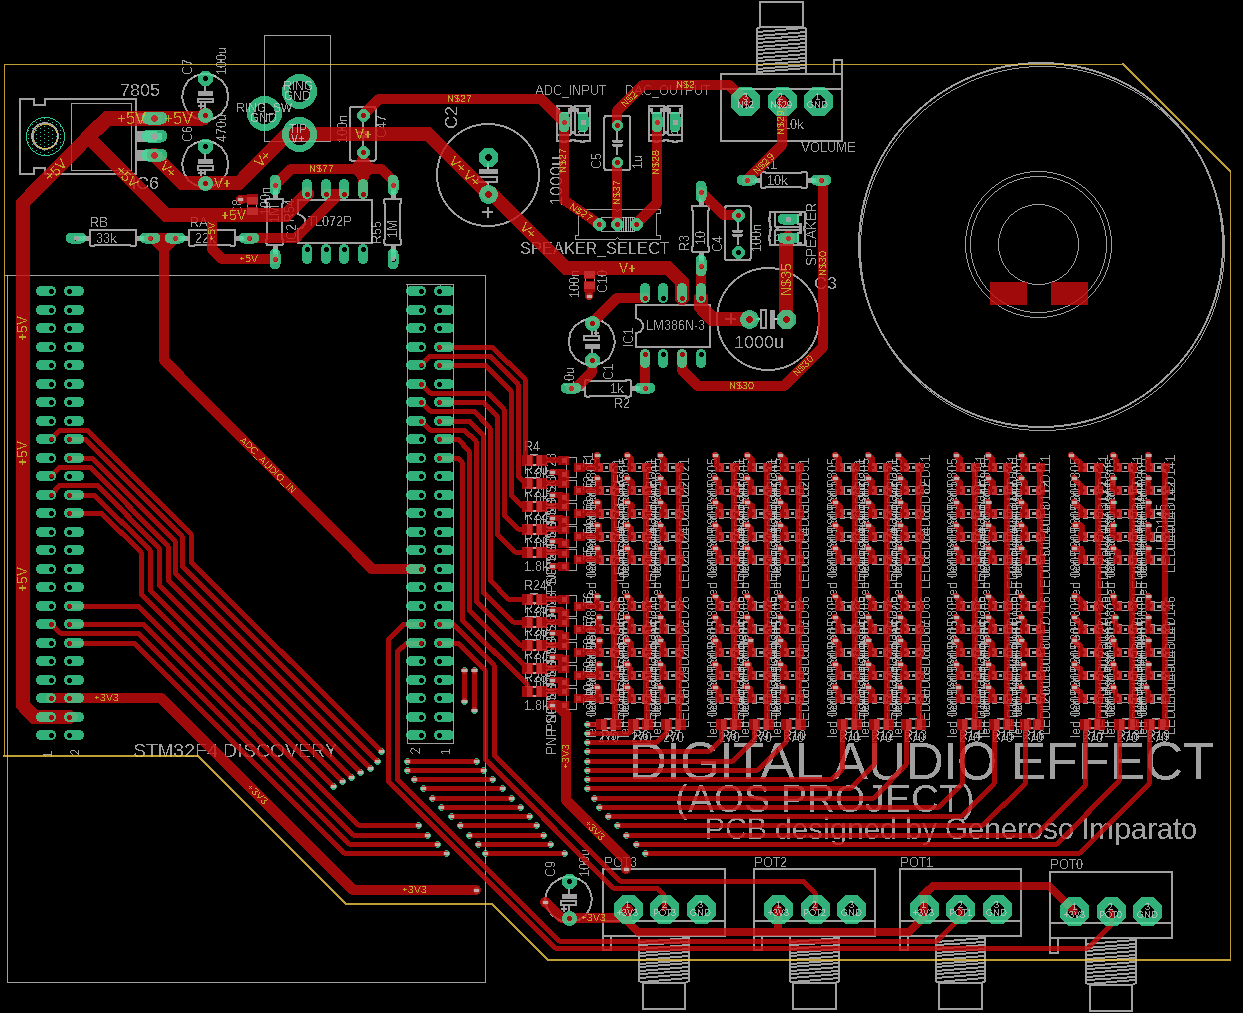
\includegraphics[width=0.8\textwidth]{img/top.png}
        \caption{top layer}
    \end{figure}
    
    \begin{figure}[H]
      \centering
        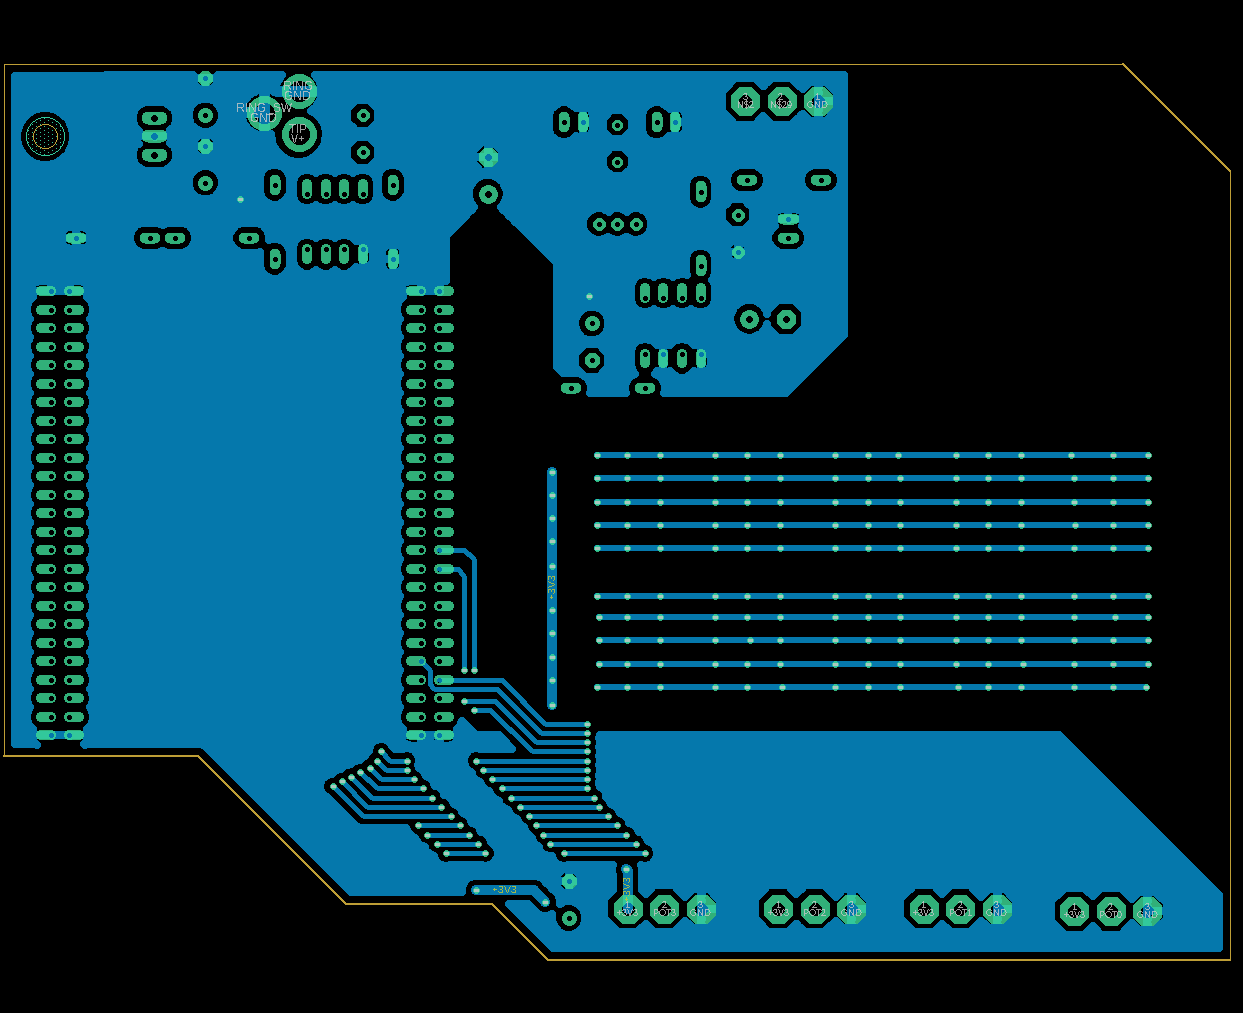
\includegraphics[width=0.8\textwidth]{img/bot.png}
        \caption{bottom layer}
    \end{figure}
    
    \newpage
    
    \subsubsubsection{Renderings}
    
    \begin{figure}[H]
      \centering
        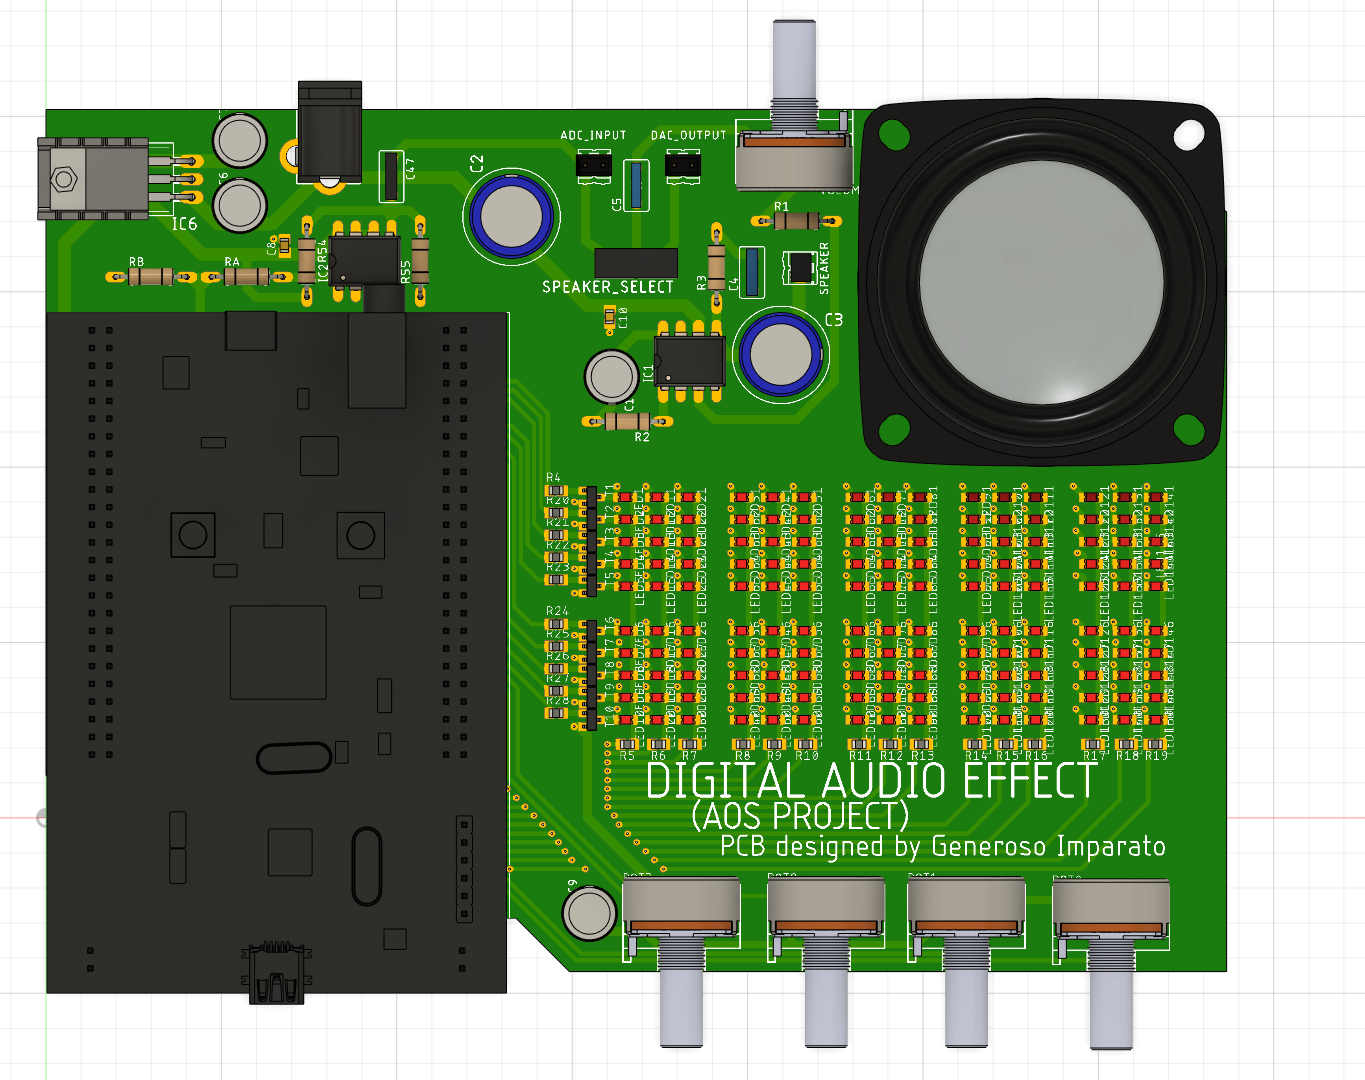
\includegraphics[width=\textwidth]{img/pcb1.png}
    \end{figure}
    
    \begin{figure}[H]
      \centering
        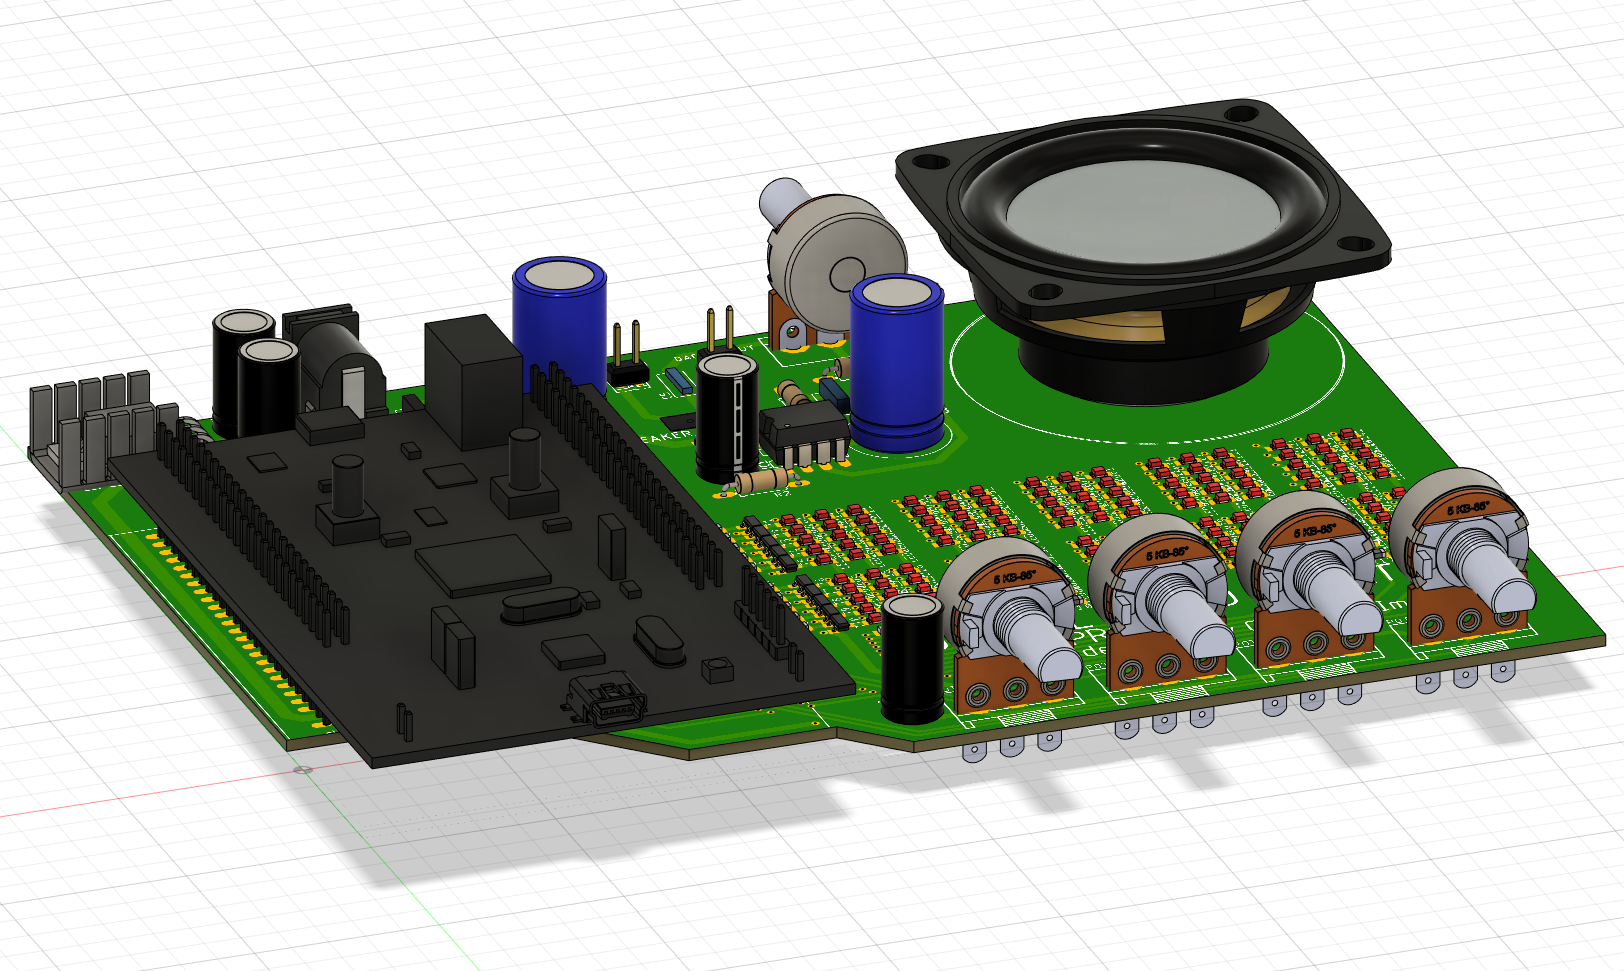
\includegraphics[width=\textwidth]{img/pcb2.png}
    \end{figure}
    
    \vfill

\subsection{Software}
\label{sec:SW}
In this section we describe the real-time OS utilized, the structure of our code in terms of optimizations and scalability, as well as our design choices regarding the management of the various threads and the implementation of different drivers.\\
Finally, we talk about the digital audio effects and their implementation in detail.
    
\subsubsection{Miosix}
\label{sec:Miosix}

Miosix is an embedded OS kernel developed by Federico Terraneo designed to run on 32bit microcontrollers, especially on STM32, EFM32 and LPC2000 microcontroller families. \par

It is used for real-time operating applications and provides operative system abstraction layers such as single process, multi-threading and multi-process (experimental). \par

There is also support for the standard POSIX thread API (threads, mutexes and condition variables) other than full support for C and C++ standard libraries. The Miosix kernel is licensed under the GPL license.

\subsubsubsection{OS Choice}

This project heavily relies on multi-threading and real-time management, so this OS was a good fit, since it supports multi-threading natively, as well as synchronization mechanisms.\par

Another advantage is the small code size, fundamental for limited flash memory as in the case of most microcontrollers.


\subsubsection{Multi-threading Design}
\label{sec:Thread}

\begin{figure}[H]
    \begin{figure}[H]
    \centering
        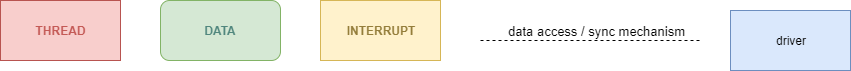
\includegraphics[width=\textwidth]{img/legenda.png}
        \caption{Diagram Legenda}
    \end{figure}
        
    \centering
        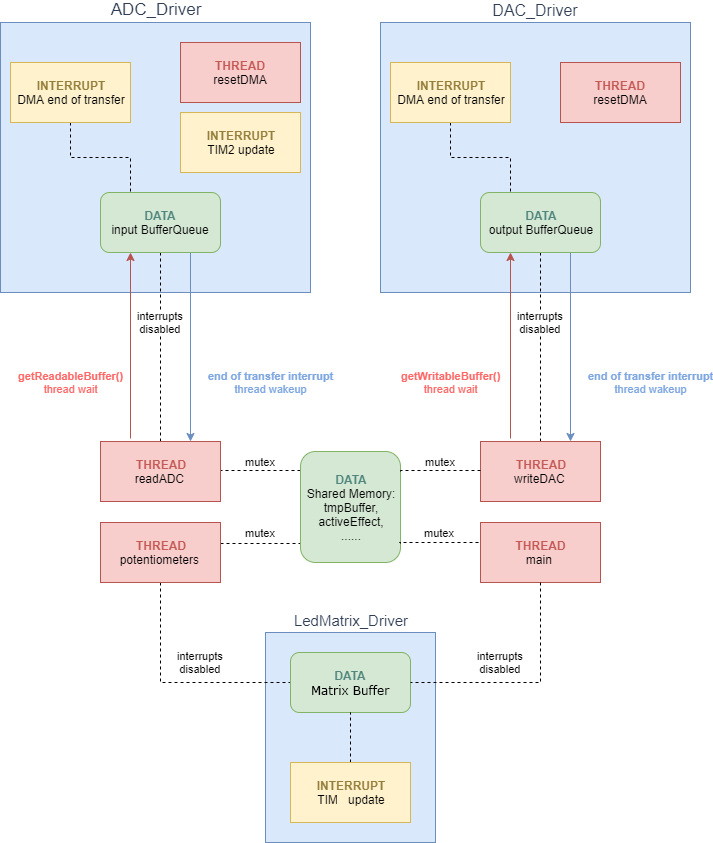
\includegraphics[width=\textwidth]{img/threads_.png}
        \caption{Threads, interrupts and data access relationships}
\end{figure}
        
\newpage

The application is realized with 6 threads.
The two most important threads \code{readADC} and \code{writeDAC} have the highest priority because they should be responsive to allow the audio stream without lags or skipping buffers.\par
\code{readADC} reads from a buffer queue in the \code{ADC\_Driver}, which is filled with audio sampled from ADC at 44,1 kHZ, in a similar way \code{writeDAC} writes in the buffer queue of the \code{DAC\_Driver}.\\
When \code{getReadableBuffer()} is called the \code{readADC} thread is put in a wait state until a buffer is available to be read, when the DMA has finished the transfer.\\
In a similar way, when \code{getWritableBuffer()} is called, the \code{writeDAC} thread is put in wait until a buffer is available to be wrote. \par

In order for the threads to be synchronized, it is required that the samples in input, and the ones in output are read/wrote at the same frequency, which in this case is 44,1 Khz, because it is a standard sampling frequency for audio. \\
The input/output buffer queues are accessed by interrupts (DMA) and threads (\code{readADC}/\code{writeDAC}), so to avoid concurrency problems, interrupts are disabled when accessing from the thread.\par

The potentiometer and main thread spin at fixed rates and are responsible for reading potentiometers values from the ADC and for checking the button to switch effect/audio source.\par

The two \code{resetDMA} threads are responsible to restart the DMAs in case the process stops because no buffer was available to be read/wrote.

    
% \newpage
    
\subsubsection{Drivers}
\label{sec:Drivers}
In order to hide the low level handling of peripheral registers and the logic required, we wrote some classes that act as drivers, providing higher level methods to use the ADC, DAC and Led Matrix.
The drivers are implemented as static classes.


\subsubsubsection{TIMx Configuration}
\label{sec:TIMx}

Since drivers use hardware timer interrupts, we will show how the right frequency of the interrupts is obtained. \par

Starting from the internal clock frequency ($168 MHz$), we pass through the AHB Prescaler and the AHB1 Prescaler, so the initial timer frequency is:

$$f_{TIMx} = \frac{f_{clk,int}}{AHB\_PSC \cdot APB1\_PSC} = \frac{168MHz}{4} =  42Mhz$$


Then, the frequency can be further prescaled setting the 16 bit prescaler (TIMx\_PSC) and the auto-reload register (TIMx\_ARR), according to this formula:

$$f_{event} = \frac{f_{TIMx}}{(TIMx\_PSC+1)\cdot(TIMx\_ARR+1)}$$

    
\subsubsubsection{ADC Driver}
\label{sec:ADC}
The peripherals used by the driver are ADC1, ADC2, TIM2, DMA2.\par
ADC2 is configured in DMA mode, single conversion triggered from the TIM2 update event and the channel is connected to the audio buffer input circuit.\par

TIM2's update frequency is set according to this formula, which was explained in the \nameref{sec:TIMx} section:

$$f_{update} = \frac{f_{TIM2}}{(TIM2\_PSC+1)\cdot(TIM2\_ARR+1)} = \frac{42MHz}{(16+1)\cdot(55+1)} = 44.1kHz$$

DMA2 is set in peripherals to memory mode to fill \code{AUDIO\_BUFFERS\_SIZE} number of samples of the input buffer queue.\par
    
The ADC resolution is 12 bits, so the values of the samples are in range from $0$ to $2^{12}-1 = 4095$
    
The driver acts like a \textit{producer} of audio buffers in the input queue.
If the queue is full and a new buffer cannot be added, the DMA stops, so there is a thread that spins in the background to restart the DMA as soon as the queue is free again.
  

\code{ADC\_Driver} provides access to the reader thread through the following method: \\
\begin{lstlisting}
const unsigned short* ADC_Driver::getReadableBuffer(miosix::Thread* readerThread) 
\end{lstlisting}
The reader thread is set in wait state if a buffer is not available to be read, it will be woken up later, when the DMA end of transfer interrupt occurs and the buffer is filled again.\par
    
The driver has also methods to perform single ADC conversions or multiple conversions with a low pass filter.
For these functionalities ADC1 is used:\\
\begin{lstlisting}
unsigned short ADC_Driver::singleConversion(unsigned short channel);
unsigned short ADC_Driver::filterConversions(unsigned short channel);
\end{lstlisting}
    
\subsubsubsection{DAC Driver}
\label{sec:DAC}
The DAC used is the CS43L22, which is already mounted on the discovery board.\\
It operates in I2S mode, for which the SPI3 peripheral is used with the internal audio PLL set to 44,1 kHz.\\
DMA1 is set in memory to peripheral mode to send \code{AUDIO\_BUFFERS\_SIZE} number of samples from the the output buffer queue to the DAC through I2S.\\  
I2S protocol uses 16 bit unsigned PCM samples, so the values are in range from $0$ to $2^{16}-1 = 65535$\par

The driver acts like a \textit{consumer} of audio buffers in the output queue.
If there is no buffer available in the queue, the DMA stops, so there is a thread that spins in the background to restart it as soon as the queue is filled again.
    
\code{DAC\_Driver} provides access to the writer thread through the following method: \\
\begin{lstlisting}
unsigned short * DAC_Driver::getWritableBuffer(miosix::Thread* writerThread)
\end{lstlisting}
The writer thread is set in wait state if a buffer is not available to be wrote, it will be woken up later, when the DMA end of transfer interrupt occurs and the queue is free again.\par
    
The DAC output is connected to audio jack on the discovery board, which is then connected to the speaker amplifier on the main PCB with a jack cable.
    
    
\subsubsubsection{Led Matrix Driver}
\label{sec:LED}
The Led Matrix serves as the output viewer of this project.
To better handle this component, \code{Led\_Matrix\_Driver} was implemented. \par

\code{Led\_Matrix\_Driver} provides access to the writer thread through the following method: \\
\begin{lstlisting}
void LedMatrix_Driver::setString(const std::string &str);
\end{lstlisting}

This method writes the led values in a buffer according to the string given as input. \\
To write in the buffer, a \code{FastInterruptDisableLock} is needed to avoid concurrency problems with respect to the other threads which access this method. \par
Then, the method \\

\begin{lstlisting}
void LedMatrix_Driver::writeLeds();
\end{lstlisting}
lights up the leds based on the buffer's values, \textit{one row at a time}.


As we can see in the \nameref{sec:Circuit} section of the PCB, there are PNP transistors only for the rows, so we can light up at most one entire row to avoid damaging the board, since the maximum current output allowed by the board is $100 mA$. \\
Running this on a separate thread was not a good choice, since the other threads affected its behaviour in a visible manner, so we chose to implement an \textit{Interrupt Routine} to achieve a constant refresh rate of the led matrix.\\
So we used an internal timer (TIM5) to trigger the IRQ.
First of all, we configured TIM5's frequency according to this formula, which was explained in the \nameref{sec:TIMx} section:

$$f_{update} = \frac{f_{TIM5}}{(TIM5\_PSC+1)\cdot(TIM5\_ARR+1)} = \frac{42MHz}{(349+1)\cdot(239+1)} = 500Hz$$

This means that each row of leds is refreshed in such a way that we can see all of the rows active at the same time.\\
Note that, since an Interrupt call refreshes a single row of the led matrix, lowering the frequency value makes the view unstable.\par



\subsubsection{Audio Chain}
The audio chain is mainly implemented in the \code{readADC}/\code{writeDAC} threads.\\
\code{readADC} thread copies buffers from the \code{ADC\_Driver} into a shared buffer, which is accessed with mutex protection because it is also used by \code{writeDAC} thread.\\ It also converts values from unsigned 12 bit to floating point.\\
\code{writeDAC} is the thread that performs the actual DSP on the buffer, before writing it to the \code{DAC\_Driver}.\par

If the audio source is set to \code{ADC}, the shared buffer is used as input for the active effect DSP algorithm.\\
If the audio source is set to \code{Synthesizer} the shared buffer is not used, because input samples are generated by the thread and then fed into the active DSP algorithm.\\
Then samples are converted from floating point to unsigned 16 bit PCM and sent to the \code{DAC\_Driver}.\\
The number of samples in each buffer can be changed by defining \code{AUDIO\_BUFFERS\_SIZE}, which is currently set to 512.

\subsubsection{DSP Effects}

The synth and the DSP effects are all implemented by extending a base class \code{AudioEffect}, that provides virtual methods that can be overridden to create different effects.\\ 
In particular the DSP algorithm is executed in the method:\\
\begin{lstlisting}
virtual void AudioEffect::writeNextBuffer(float* inBuff, float* outBuff);
\end{lstlisting}
The default implementation just copies \code{inBuff} into \code{outBuff}, applying no effect.\par

This design allows to easily implement different effects, focusing only on the DSP part and avoiding to handle all the audio chain, as well as the controls updating from the potentiometers.\par

The effects included in this demonstration are a \textit{Delay}, a \textit{Filter} and a \textit{Tremolo}.

\subsubsubsection{Delay}
The delay effect is obtained thanks to a circular buffer, which is continuously refilled from the beginning once is full.\\
This buffer has a size that is a multiple of \code{AUDIO\_BUFFERS\_SIZE}, and it is used to keep in memory samples from past buffers.\\
When producing the next buffer, samples from the delay buffer are added to the input, multiplied by a feedback parameter.\\
The maximum delay time depends on the size of the circular buffer, and can be computed as:
$$T_{max} = \frac{buffer\_size}{f_{sampling}}$$
In this case, the circular buffer size is set to:
$$T_{max} = \frac{k\cdot\code{AUDIO\_BUFFERS\_SIZE}}{44.1  kHz} = \frac{45\cdot512}{44.1  kHz} = 522 ms$$

The actual delay time, as well as the feedback are left as parameters controllable with potentiometers.

\subsubsubsection{Filter}
The filter effect implements a simple low-pass, band-pass and high pass filter.\\
Controllable parameters are cutoff frequency and resonance. \\
The DSP algorithm implemented is from Paul Kellett and can be found at:  \\
https://www.musicdsp.org/en/latest/Filters/29-resonant-filter.html


\subsubsubsection{Tremolo}
The tremolo effect applies a modulation on the signal amplitude, which is controlled by a software LFO (low frequency oscillator).\\
The signal samples are multiplied by a factor which is generated by the LFO and the speed can be controlled as parameter.

\subsubsubsection{Synthesizer}
We added a wavetable synthesizer to be used as an audio source.\\
it is implemented by extending the \code{AudioEffect} class in a way similar to the DSP effects, but since it generates the samples from scratch it does not read from \code{inBuffer}, but writes to \code{outBuffer}.\par

Wavetables are pre-computed to make the real-time computations faster, so when the samples are generated, values from the wavetables are used, with proper stretching according to the desired sound frequency.\par

The synthesizer has 3 independent oscillators, each one using a different wavetable: 
\begin{itemize}
    \item Sine
    \item Triangle
    \item Square Wave
\end{itemize}

Those waveforms are added together and multiplied by the respective amplitude, in order to generate the output samples. \\
Each individual oscillator and its parameters can be controlled with potentiometers.

\newpage

Controllable parameters are:
\begin{itemize}
    \item Frequency
    \item Amplitude
    \item Speed
    \item Mode
\end{itemize}

\textit{Speed} parameter controls the speed at which the selected pattern is played.\\
\textit{Mode} allows to select a pattern for the oscillator, such as continuous note, scale, random notes, octaves and so on. \\


\section{Conclusions}
This project covered the development of a system in which multiple audio sources could go through different digital audio effects, all in a real-time environment and with an enhanced user experience brought by a custom PCB.\par

We experienced some noise in the audio sampled from ADC, and we couldn't remove it completely, but overall, we can say that our initial goal was reached and we built a solid base for future improvements.\par

The \code{AudioEffect} class is very easy to extend, so adding a new digital audio effect and viewing it in the led matrix, is a very simple task, and this applies also to adding other audio sources.


\subsection{Future Improvements}

We could implement audio effects which require the usage of a FFT to expand the pool of options.\par
Another possible improvement would be adding an anti-aliasing filter on the audio signal before the ADC sampling, which could maybe solve the noise problem mentioned before.\par
Also, we could use a cleaner power supply and a better analog/digital power separation on the PCB.\par
Finally, an improvement to the user experience would be a better handling of controls shown in the led matrix.


\end{document}